\documentclass[a4paper,fontsize=10pt,italian,pdftex]{scrartcl}

% FONT, INPUT, BABEL
\usepackage[italian]{babel}
\usepackage[T1]{fontenc}
\usepackage[utf8x]{inputenc}
\usepackage[activate,tracking,spacing]{microtype}
\usepackage{lmodern}
\usepackage[a4paper]{geometry}
\microtypecontext{spacing=nonfrench}

% ALTRO
\usepackage{amsmath,amsfonts,amsthm,amssymb,mathrsfs,textcomp,wasysym}
\usepackage[pdftex]{graphicx}
\usepackage{subfig}
\usepackage{url}
\usepackage{indentfirst}

% MACRO
\newcommand{\dd}[1]{\mathrm{d}#1}
\newcommand{\ddt}[1]{\frac{\dd #1}{\dd{t}}}
\newcommand{\pdd}[2]{\dfrac{\partial #1}{\partial #2}}
\newcommand{\Flux}{\mathbf{F}}
\newcommand{\NumFlux}{\mathbf{\mathcal{F}}}
\newcommand{\nn}{\hat{\mathbf{n}}}
\newcommand{\abs}[1]{\left| #1 \right|}
\DeclareMathOperator{\diverg}{div}
\DeclareMathOperator{\diam}{diam}

% PDF
\usepackage[bookmarks=true,pdftex,unicode,hypertexnames=false,pdfborder={0 0 0}]{hyperref} 
\hypersetup{
pdfauthor = {Simone Pezzuto e Daniela Martelli},
pdftitle = {Implementazione in C++ di un codice 2D per la risoluzione di leggi di conservazione non lineari},
pdfsubject = {Progetto nell'ambito del corso di Programmazione Avanzata e Calcolo Scientifico per la Fluidodinamica}}

% BIBLIO
\usepackage{amsrefs}

%STILE
\setkomafont{caption}{\small}
\setkomafont{captionlabel}{\small\bfseries\sffamily}

%LISTATI
\usepackage{color}
\definecolor{commenti}{rgb}{0.13,0.55,0.13}
\definecolor{stringhe}{rgb}{0.63,0.125,0.94}
\usepackage{listings}
\lstloadlanguages{C++}
\lstset{basicstyle = \scriptsize,
keywordstyle = \bfseries \color{blue},
identifierstyle =,
numbers=left,stepnumber=1,numberstyle=\tiny,tabsize=3,
commentstyle = \color{commenti},
stringstyle = \ttfamily \color{stringhe},
showstringspaces = false, % no special string spaces
%emph = {for, if, then, else, end},
%emphstyle = \color{blue},
firstnumber = auto, % numero della prima linea
language = {C++}, % per riconoscere la sintassi matlab
extendedchars = true, % per abilitare caratteri particolari
breaklines = true, % per mandare a capo le righe troppo lunghe
breakautoindent = true, % indenta le righe spezzate
breakindent = 30pt, % indenta le righe di 30pt
}

\begin{document}
\nocite{*}
% INTESTAZIONE
\begin{center}
\rule{\textwidth}{0.1mm}
\LARGE\sffamily{\bfseries{Implementazione in C++ di un codice 2D per la risoluzione di leggi di conservazione non lineari}}
\rule[0.4cm]{\textwidth}{0.1mm}

\begin{minipage}{0.4\textwidth}
\begin{center}
\Large
Daniela Martelli\\ \small
(Matr. \textbf{721891})
\end{center}
\end{minipage}
\begin{minipage}{0.4\textwidth}
\begin{center}
\Large
Simone Pezzuto\\ \small
(Matr. \textbf{724680})
\end{center}
\end{minipage}

\vspace{0.5cm}
\itshape\large Settembre 2009
\vspace{0.5cm}

\end{center}
% FINE INTESTAZIONE
\begin{abstract}
\small
Lo scopo di questo progetto è implementare in C++ il metodo dei Volumi Finiti per la risoluzione di leggi di conservazione non lineari in due dimensioni su griglie non strutturate.

In questo report, dopo una breve introduzione alle leggi di conservazione e al metodo dei Volumi Finiti, cercheremo di descrivere la struttura del codice \texttt{ConservationLaw2D} ponendo particolare enfasi alle scelte effettuate nel corso dello sviluppo.

In particolare ci soffermeremo sugli aspetti algoritmici legati alle principali difficoltà incontrate, come la gestione di una mesh non strutturata o la possibilità di rendere modulare il codice, mentre delegheremo la descrizione delle procedure più standard alla documentazione interna.

Infine nell'ultima parte forniremo due esempi applicativi sul funzionamento del codice: il primo, con il modello delle onde in acque basse, riguardante il crollo di una diga (\emph{Dam Break Problem}), mentre il secondo, con il modello di Eulero, riguarderà l'interazione di un'onda di shock con una bolla (\emph{Shock Bubble Problem}).
\end{abstract}
\section{Leggi di conservazione non lineari}
\subsection{Formulazione integrale e differenziale}
Una generica legge di conservazione si può scrivere in forma integrale come:
\begin{equation} \label{eq:conslawintegrale}
\int_\omega \pdd{\mathbf u}{t} \: \dd{x} + \oint_{\partial \omega} \Flux \cdot \nn \: \dd{\gamma}
= \int_\omega \mathbf S \: \dd{x}
\end{equation}
dove $\omega \subset \Omega \subseteq \mathbb{R}^d$, $d=1,2,3$, è un \emph{volume di controllo} arbitrario all'interno del dominio $\Omega$ nel quale si studia il problema, $\mathbf u = \mathbf{u}(x,t)$ è il vettore delle $m$ variabili conservate, $\Flux = \Flux(\mathbf u)$ è il tensore di flusso attraverso $\partial \omega$ ed infine $\mathbf S = \mathbf S(\mathbf u, x, t)$ è un'eventuale sorgente esterna.

L'equazione \eqref{eq:conslawintegrale} esprime in termini matematici il fatto che la variazione di $\mathbf u$ all'interno di $\omega$ è pari al flusso netto attraverso il bordo più un eventuale termine sorgente.
 
Spesso la legge di conservazione si esprime in termini differenziali:
\begin{equation} \label{eq:conslawdiff}
\begin{cases}
\; \pdd{\mathbf u(x,t)}{t} + \diverg \Flux(\mathbf u) = \mathbf S(\mathbf u,x,t) & \text{con $x \in \Omega$, $t > 0$} \\[1ex]
\; \mathbf{u}(x,0) = \mathbf u_0(x) \\[1ex]
\; \text{+ condizioni al bordo}
\end{cases}
\end{equation}

Tale formulazione è ragionevole a patto di garantire sufficiente della soluzione $\mathbf u$. Purtroppo nelle leggi di conservazione non lineari è lecito aspettarsi soluzioni discontinue, indipendentemente dalla regolarità dei dati iniziali: in questi casi il problema differenziale \eqref{eq:conslawdiff} perde di significato lungo le discontinuità e si deve far riferimento a \eqref{eq:conslawintegrale}.
 
Il sistema \eqref{eq:conslawdiff} si può scrivere in forma quasi-lineare sviluppando le derivate nel termine di divergenza. Ad esempio con $\Omega \subset \mathbb{R}^2$ e $\Flux = \begin{bmatrix} \Flux_1 & \Flux_2 \end{bmatrix}$ si ha:
\begin{equation}\label{eq:conslawquasilin}
\pdd{\mathbf u(x,t)}{t} + \mathbf{A}_1(\mathbf{u}) \pdd{\mathbf u}{x_1} + \mathbf{A}_2(\mathbf{u}) \pdd{\mathbf u}{x_2} 
= \mathbf 0
\end{equation}
dove si è posto $\mathbf{A}_i(\mathbf{u}) = \pdd{\Flux_i(\mathbf{u})}{\mathbf u}$ e, per comodità, $\mathbf S \equiv \mathbf 0$.

\subsection{Soluzioni ad onde piane}
Le soluzioni ad \emph{onde piane} per il sistema \eqref{eq:conslawquasilin} rivestono un ruolo particolarmente interessante: supponiamo di partire con un dato iniziale $\mathbf u(x,0) = \mathbf{u}_0 (\xi)$, con $\xi = x \cdot \nn$, cioè consideriamo una funzione che varia solo in direzione $\nn$, e chiediamoci se è possibile avere una soluzione del tipo $\mathbf u(x,t) = \mathbf{u}(\xi-\lambda t)$.

Affinché sia possibile $\lambda$ dev'essere un autovalore di $\mathbf{A}(\mathbf{u}; \nn) := \mathbf{A}_1(\mathbf{u}) n_x + \mathbf{A}_2(\mathbf{u}) n_y$ e $\mathbf{u}$ il corrispondente autovettore. Quindi, se $\mathbf{A}(\mathbf{u}; \nn)$ è diagonalizzabile con autovalori reali allora è possibile trovare una soluzione ad onde piane. Infatti in questo caso il sistema \eqref{eq:conslawquasilin} diventa:
\begin{equation} \label{eq:conslawondepiane}
\pdd{\mathbf{u}}{t} + \mathbf{A}(\mathbf{u};\nn) \pdd{\mathbf u}{\xi} = \mathbf{0}
\end{equation}
 
L'equazione \eqref{eq:conslawondepiane}, che si può riscrivere in modo equivalente come:
\begin{equation*}
\pdd{\mathbf{u}}{t} + \pdd{}{\xi} \Flux(\mathbf{u};\nn) = \mathbf{0}
\end{equation*}
con $\Flux(\mathbf{u};\nn) = \Flux(\mathbf{u}) \cdot \nn$, risulterà fondamentale nel momento in cui verrà implementato il metodo dei Volumi Finiti su griglie non strutturate, in quanto suggerisce come discretizzare il problema in modo da trovare un adeguato flusso numerico lungo una direzione $\nn$ data.
 
\subsection{Problema di Riemann}
Tra le soluzioni ad onde piane risultano particolarmente importanti quelle che soddisfano il problema di Riemann:
\begin{equation} \label{eq:conslawriemann}
\begin{cases}
\pdd{\mathbf u}{t} + \pdd{}{\xi}\Flux(\mathbf u; \nn) = \mathbf 0 & \text{con $\xi \in \mathbb{R}$, $t > 0$} \\[1.2ex]
\mathbf{u}(\xi,0) = \begin{cases} \mathbf u_L & \text{per $\xi < 0$} \\ \mathbf u_R & \text{per $\xi > 0$} \end{cases}
\end{cases}
\end{equation}
Il sistema, a tutti gli effetti monodimensionale, si può studiare in dettaglio fissata $\Flux(\mathbf u; \nn)$: in particolare si può far ricorso a tutta la teoria per sistemi di equazioni non lineari 1D.

Dalla stretta iperbolicità di $\mathbf{A}(\mathbf{u};\nn)$ possiamo trovare sempre un insieme $\bigl\{ \lambda_1, \ldots, \lambda_m \bigr\}$  di $m$ autovalori e un insieme di $m$ autovettori corrispondenti $\bigl\{ \mathbf{r}_1, \ldots, \mathbf{r}_m \bigr\}$, ed è possibile mostrare che il problema di Riemann \eqref{eq:conslawriemann} ha una soluzione che consiste in $m+1$ stati costanti i quali possono essere connessi da shocks, onde di rarefazione o discontinuità di contatto \cite{Kroner97}.

In generale per il problema di Riemann \eqref{eq:conslawriemann} la soluzione non è unica: nascono a questo proposito diverse condizioni, dette di \emph{entropia}, che se soddisfatte garantiscono in una certa misura che la soluzione trovata sia quella fisicamente più ragionevole.

Da un punto di vista numerico il problema si pone nel momento in cui si cerca di approssimare la soluzione, perché il metodo che si utilizza potrebbe non garantire a priori la convergenza alla soluzione entropica. La situazione tipica è la presenza di un'onda di shock al posto di un'onda di rarefazione.
\section{Il metodo dei Volumi Finiti su griglie non strutturate}
Consideriamo un'approssimazione poligonale $\Omega_h$ di $\Omega$, e costruiamone una triangolazione $\mathcal{T}$, ossia un insieme di poligoni chiusi $K_i$, $i=1,\ldots,N$, tale che:
\begin{enumerate}
\item $\Omega_h = \bigcup_{i=1}^N K_i$;
\item Dati $K_i$, $K_j$ con $i\neq j$, sia $K_i \cap K_j = \varnothing$ oppure $K_i \cap K_j$ è un vertice o un lato comune ai due elementi.
\end{enumerate}

L'idea che sta alla base del metodo dei \emph{Volumi Finiti} è quella di considerare la formulazione integrale relativa all'equazione \eqref{eq:conslawintegrale} ponendo $\omega = K_i$:
\begin{equation*}
\ddt{} \int_{K_i} \mathbf u \: \dd{x} + \oint_{\partial K_i} \Flux \cdot \nn \: \dd{\gamma}
= \int_{K_i} \mathbf S \: \dd{x}
\end{equation*}
A questo punto, per $t$ fissato, approssimiamo la soluzione numerica e il temine sorgente come costanti all'interno di ogni elemento $K_{i}$:
\begin{equation*}
\mathbf{U}_i(t) \approx \frac{1}{\abs{K_i}} \int_{K_i} \mathbf u(x,t) \: \dd{x}, \qquad
\mathbf{S}_i(t) \approx \frac{1}{\abs{K_i}} \int_{K_i} \mathbf S(\mathbf{u},x,t) \: \dd{x}
\end{equation*}
Sostituendo si ottiene:
\begin{equation} \label{eq:odefvm}
\ddt{\mathbf{U}_i(t)} = - \frac{\abs{e_{ij}}}{\abs{K_i}} \sum_{e_{ij} \in \partial K_i} \NumFlux(\mathbf U_i, \mathbf U_j, \nn_{ij}) + \mathbf{S}_i(t)
\end{equation}
dove $e_{ij}$ è il lato condiviso dagli elementi $K_i$ e $K_j$ e:
\begin{equation*}
\NumFlux(\mathbf U_i, \mathbf U_j, \nn_{ij}) := \frac{1}{\abs{e_{ij}}} \oint_{e_{ij}} \Flux \cdot \nn_{ij} \: \dd{\gamma}
\end{equation*}
è il \emph{flusso numerico} attraverso il lato di normale $\nn_{ij}$ (cioè la normale esterna al lato $e_{ij}$ diretta da $K_i$ a $K_j$), calcolato utilizzando i valori della soluzione a destra e a sinistra dell'interfaccia stessa. Esempi di vari flussi numerici si possono trovare nell'Appendice \ref{app:flussinum}.

Utilizzando Eulero esplicito per risolvere \eqref{eq:odefvm} si ottiene il classico \emph{schema a Volumi Finiti}:
\begin{equation} \label{eq:schemavolumifiniti}
\mathbf{U}_{i}^{n+1} = \mathbf{U}_{i}^{n} - \Delta t \sum_{e_{ij} \in \partial K_i} \frac{\abs{e_{ij}}}{\abs{K_i}} \NumFlux(\mathbf U^n_i, \mathbf U^n_j, \nn_{ij}) + \mathbf{S}_{i}(\mathbf U^n_{i})
\end{equation}
Osserviamo che il valore della soluzione $\mathbf{U}_i$ è assegnata all'intero elemento $K_i$, e non ad uno specifico nodo. Essendo un'approssimazione di ordine zero, si è soliti assegnare questo valore ad un punto interno di $K_i$, tipicamente al baricentro. Questo tipo di discretizzazione è detta \emph{cell-centered}. Dato che i vertici non entrano in gioco direttamente può diventare problematico assegnare condizioni al bordo essenziali, mentre l'assegnazione di condizioni di flusso è affrontata in modo naturale.

Un'alternativa è invece quella di costruire una triangolazione \emph{duale}, composta da poligoni centrati nei vertici della triangolazione originale (per esempio da una triangolazione Delaunay si utilizza come duale il diagramma di Voronoi). Il problema integrale si discretizza quindi sulla triangolazione duale, cosicché assegnando la soluzione al centro dei poligoni si sta automaticamente costruendo la soluzione nei vertici della triangolazione originale. Si può così ovviare al problema delle condizioni al bordo essenziali poiché adesso i nodi al bordo sono ``elementi'' della triangolazione duale. Questo tipo di discretizzazione è detta \emph{vertex-centered}.

\section{Implementazione del codice in C++}
Per la risoluzione di leggi di conservazione non lineari 2D su griglie triangolari è stata sviluppata la libreria \texttt{ConservationLaw2D}, in gran parte scritta in C++.

Il codice permette di risolvere problemi basati su diversi tipi di modelli, con particolar riguardo alle equazioni di Eulero 2D. Non mancano però esempi sulle equazioni dell'acustica o di onde in acque basse. Inoltre è possibile estendere il codice ad altri modelli o metodi di risoluzione (come Discontinous Galerkin) con relativa semplicità.

La struttura del codice si organizza essenzialmente su in tre parti distinte:
\begin{enumerate}
\item La gestione della mesh;
\item La descrizione del modello (Eulero ad esempio);
\item Il solutore (Volumi Finiti).
\end{enumerate}

\subsection{La gestione della mesh}
La parte più sostanziosa e certamente meno banale è quella riguardante la gestione della mesh. 

Il requisito essenziale nel nostro caso riguarda la possibilità di effettuare particolari ``query'' sulle relazioni tra i vari elementi. Questo tipo di problema può essere risolto in svariati modi, ma ognuno è un compromesso tra utilizzo di memoria ed efficienza.

Ad esempio, alcuni tipi di query possono essere:
\begin{itemize}
\item Dato un vertice, quali sono i poligoni ad esso adiacenti, ossia quali poligoni hanno tra i propri vertici quello in questione? 
\item Dato un poligono, quali sono i poligoni ad esso adiacenti, cioé che condividono con esso un lato? 
\item Dato un lato, quali sono i poligoni che insistono su di esso? 
\end{itemize}

Gli oggetti che compongo una mesh sono gli elementi, i lati e i vertici. Ognuno è collegato all'altro secondo relazioni di appartenenza, per esempio un lato è formato da due vertici, e un poligono è un insieme di lati. Quindi se volessi sapere quali sono i vertici del poligono basterebbe scorrere sui lati e restituire i vertici. Già in questo caso molto semplice però vi sono difficoltà: il lato non è in genere orientato, quindi quale dei due vertici considerare? Un triangolo ha 3 lati, quindi dei 6 vertici forniti da questi ultimi 3 saranno coincidenti, ma non è a priori stabilita una regola per recuperare una lista di vertici unici (magari anche in ordine antiorario).

Sono inoltre molto complesse (e quindi dispendiose in termini computazionali) query che devono risolversi in ordine inverso, per esempio recuperare i poligoni adiacenti ad un vertice. In teoria dovrei scorrere tutti i poligoni della mesh e per ognuno scorrere i vertici, e fare poi un confronto.

Riassumendo dunque, cerchiamo una struttura dati che non soffra troppo nella risoluzione di query di adiacenza, che fornisca un certo orientamento ai lati e che magari non sia dispendiosa in termini di memoria.

La struttura dati che abbiamo deciso di adottare è di tipo \emph{half-edge}, dove ogni lato è memorizzato come coppia di lati gemelli orientati però in direzioni opposte. In particolare, ogni elemento è descritto da una successione in senso antiorario di half-edge, ognuno dei quali ha un puntatore al suo successivo, al vertice di origine, all'elemento alla sua sinistra (ricordiamo che il segmento è orientato) e al suo lato gemello (se esiste), appartenente all'elemento adiacente a quel lato. Una mesh di questo tipo è detta \emph{edge-based}\footnote{Le mesh basate su half-edge sono spesso utilizzate nella Computer Grafica perché permettono anche di descrivere superficie tridimensionali. Non è però l'unica possibilità esistente, anzi ve ne sono molte altre (winged-edge, quad-edge).}.

La scelta di utilizzare questa struttura dati fornisce qualcosa che non è troppo oneroso in termini di memoria, sufficientemente efficiente e abbastanza robusto nell'eventualità di una futura estensione a tecniche di raffinamento e deraffinamento, le quali eliminando triangoli possono rendere difficoltoso l'aggiornamento della struttura delle adiacenze.

Le query anche complesse in questa topologia diventano molto semplici ed intuitive: 
\begin{itemize}
\item I vertici di un poligono si trovano partendo da un suo mezzo lato qualsiasi, restituendo il vertice di quest'ultimo per poi passare al mezzo-lato successivo, e da qui ripetere; 
\item Il poligono adiacente ad un mezzo-lato dato, che è il poligono del lato gemello al lato dato;
\end{itemize}
Non mancano però le difficoltà, infatti questa struttura dati deve essere modificata in presenza di bordi o di vertici degeneri (un vertice è degenere se è in comune a due poligoni i quali però non hanno lati in comune tra loro, come il nodo di un papillion).

La seconda scelta progettuale di rilevanza riguarda invece la possibilità di utilizzare mesh composte da poligoni di un numero di lati non necessariamente identico (quindi non necessariamente triangolari): i Volumi Finiti infatti si applicano perfettamente a prescindere dal numero di lati del volume di controllo. La struttura dati utilizzata ha permesso di implementare tale scelta senza grossi sforzi aggiuntivi.

Infine una terza importante caratteristica è la possibilità di estendere le classi che descrivono vertice, lato e poligono a proprio piacimento, senza influenzare però la struttura dati. La mesh può quindi essere puramente topologica (essenzialmente un grafo), oppure avere anche una struttura geometrica o, come nel nostro caso, una struttura di spazio funzionale, dove ogni poligono descrive anche una funzione costante (e dunque la mesh descrive una funzione costante a tratti). In questo ambito si è fatto ricorso ad un uso moderato di \emph{templates}.
\subsubsection{La struttura dati half-edge}
Iniziamo con il descrivere dettagliatamente la struttura dati utilizzata. Come accennato, la struttura dati half-edge è di tipo edge-based, quindi gran parte dell'informazione strutturale è associata ai lati.

\begin{figure}[htb]
\centering
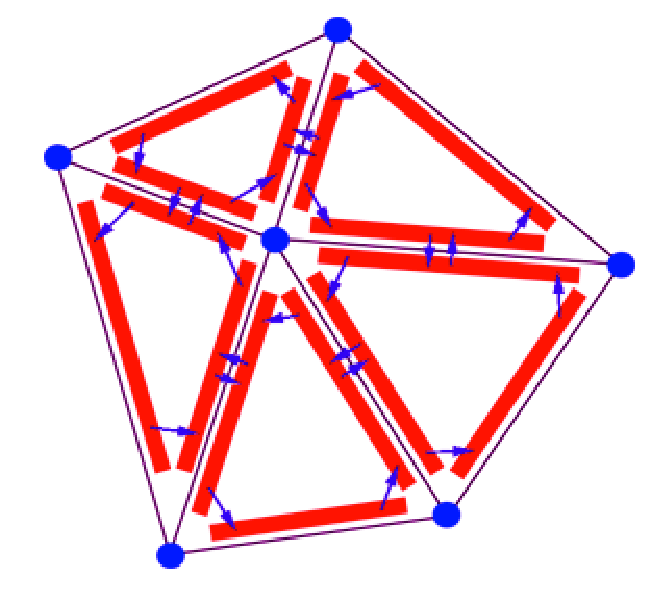
\includegraphics[width=5.8cm]{images/halfedge.pdf}
\caption{Struttura dati di tipo half-edge} \label{fig:halfedge}
\end{figure}

In Figura \ref{fig:halfedge} è rappresentato il patch di elementi di un vertice, con le relazioni esistenti tra i vari lati. L'orientamento predefinito dei lati è in senso antiorario, come si evince seguendo il senso delle frecce.

Oltre a questi puntatori, per descrivere la mesh è necessario collegare ai lati i vertici e i poligoni. Ogni vertice ha un puntatore ad uno dei lati\footnote{Come sarà spiegato più avanti, questo è in realtà falso perché sono necessarie delle modifiche per poter gestire i vertici di bordo.} che esce da esso (e viceversa ogni lato ha un puntatore al vertice d'origine), e ogni poligono ha un puntatore ad uno qualsiasi dei suoi lati (e anche in questo caso, ogni lato ha un puntatore al poligono alla sua sinistra).

Nel codice sono state definite 5 classi primitive per la struttura dati:
\begin{itemize}
\item \texttt{BaseKernel}, contenitore di tipi di dati ereditato da tutte le classi;
\item \texttt{BaseVertex}, la classe basilare del vertice, che contiene le coordinate e un puntatore ad un halfedge che da esso parte;
\item \texttt{BaseHEdge}, la classe che descrive l'halfedge, con puntatori al vertice di partenza, al lato successivo, a quello gemello e anche un puntatore al poligono alla sua sinistra. Vi sono poi metodi per accedere ai due vertici e ai due poligoni adiacenti (sempre se quello a destra esiste);
\item \texttt{BasePolygon}, la classe che descrive il poligono, contiene un puntatore ad uno dei suoi lati;
\item \texttt{BasePolygonalMesh}, ossia la mesh vera e propria che mette a disposizione iteratori sui suoi elementi (contenuti in tre liste, una per i vertici, una per i lati e una per i poligoni), nonché metodi per aggiungere nuovi poligoni e vertici.
\end{itemize}
Inoltre sia i lati che i poligoni hanno un attributo \texttt{color}, come fosse un marker che ci permette di distinguerli. Ad esempio questo ci permette di assegnare un certo valore di soluzione solo ad alcuni poligoni che abbiamo precedentemente marcato, e stessa cosa per i lati (utile nell'assegnazione delle condizioni iniziali e di bordo).
 
Tutte queste classi hanno il prefisso \texttt{Base} perché devono essere necessariamente estese, eventualmente da classi vuote (che con molta fantasia chiameremo allo stesso modo, senza il prefisso). Questo passaggio a prima vista fittizio sarà giustificato in seguito.
\paragraph{Il caso dei vertici degeneri}
Consideriamo una mesh composta da soli due triangoli i quali condividono un solo vertice. In questo caso la struttura dati non riesce a rappresentare la mesh perché partendo dal vertice e seguendo il suo puntatore ad uno dei due half-edge rimaniamo ``intrappolati'' sul triangolo indicato dal lato scelto, senza possibilità di passare a quello adiacente. In questo caso si parla di vertice degenere.

Per ovviare al problema abbiamo studiato una soluzione possibile, che per quanto macchinosa mantiene comunque tempi ragionevoli di accesso. 

L'idea è quella di salvare nel vertice la lista dei lati (e non solo uno) che si irradiano da esso. Però non è necessario avere un puntatore ad ognuno, piuttosto basta avere un puntatore ai soli lati di bordo e nell'eventualità che il vertice sia interno ad un solo lato qualsiasi.
La struttura dunque è ridondante solo nelle situazioni particolari.

\subsubsection{I circolatori}
La struttura dati descritta introduce in modo naturale il concetto di \emph{circolatore}.

È evidente ad esempio che la lista dei vertici di un poligono non ha testa né coda. Quindi partendo da un qualsiasi vertice dovrebbe essere possibile passare a quello subito successivo o precedente, eventualmente tornando su sé stesso dopo un giro completo. Pensando più in prospettiva si può quindi immaginare che anche la risposta di una query di adiacenza sia un circolatore.

Un esempio pratico di utilizzo dei circolatori è il seguente, dove per ogni vertice viene calcolata l'area media dei poligoni adiacenti.

Iniziamo con l'intestazione del codice, dove viene definito il circolatore:
\begin{lstlisting}[name=esempioCirc]
#include <mesh/mesh_default_traits.hpp>

using namespace ConservationLaw2D;

typedef Mesh::DefaultTraits<double> Traits;
typedef Traits::PolygonalMesh       SimpleMesh;

typedef SimpleMesh::vertex_it                  v_it;
typedef SimpleMesh::Vertex::PolygonCirculator  vp_cit;
\end{lstlisting}
Di seguito riportiamo invece il blocco principale:
\begin{lstlisting}[name=esempioCirc]
// Itero su tutti i vertici della mesh
for ( v_it v = mesh.v_begin(); v != mesh.v_end(); ++v ) {
    // Contatore per il numero di poligoni adiacenti
    size_t count(0);
    real_t tmparea(0.0);
    // Inizializzo il circolatore
    vp_cit p = (*v)->beginP();
    do {
        tmparea += p->area();
        count++;
        // Incremento il circolatore ...
        p++;
    // ... finche' non torno al punto di partenza
    } while( p != (*v)->beginP() );
    cout << tmparea/count << endl;
}
\end{lstlisting}
Come si può osservare una query relativamente complessa come il trovare i poligoni adiacenti al vertice dato si può scrivere con poche righe di codice, mantenendo allo stesso tempo un buon livello di astrazione. Allo stesso modo si possono trovare i lati o i vertici adiacenti al vertice dato (con i circolatori \texttt{Vertex::HEdgeCirculator} e \texttt{Vertex::VertexCirculator}). Oppure, dato un poligono, si possono cercare vertici, lati e poligoni adiacenti (rispettivamente con i circolatori \texttt{Polygon::VertexCirculator}, \texttt{Polygon::HEdgeCirculator} e \texttt{Polygon::PolygonCirculator}).

Il circolatore è definito attraverso un'unica classe \texttt{CirculatorTS}, specializzata poi attraverso l'uso di template. Si tratta di una classe generica dalla quale sono derivati tutti i circolatori possibili (escludendo quelli riferiti ai lati sono esattamente 6, elencati subito sopra). In questo modo a costo di un livello di astrazione e complessità maggiore si ha un codice molto più compatto.

La specializzazione di un circolatore avviene con una definizione del tipo (all'interno della classe \texttt{BaseVertex}):
\begin{lstlisting}
typedef typename Circulators::CirculatorTS<KERNEL,Polygon,Vertex>  PolygonCirculator;
\end{lstlisting}
dove viene definito un circolatore sui poligoni adiacenti al vertice dato. In questo modo la classe automaticamente selezionerà i metodi opportuni per circolare sui poligoni partendo da un vertice\footnote{Non essendo possibile la specializzazione parziale questa selezione avviene tramite delle variabili \emph{dummy}, una di tipo \texttt{T} e una di tipo \texttt{S} (per esempio \texttt{Polygon} e \texttt{Vertex}). I metodi necessari alla specializzazione sono quindi selezionati per overloading.}.

Essenzialmente le due procedure principali riguardando l'incremento del circolatore (cioè il passaggio all'elemento successivo) e la lettura dell'elemento corrente. Tutti i circolatori infatti non hanno un puntatore all'oggetto corrente, bensì un puntatore ad un particolare half-edge dal quale si risolve facilmente l'elemento corrente.

Sempre considerando il circolatore prima definito, la procedura di lettura ha la forma seguente:
\begin{lstlisting}
return current_hedge->polygonL();
\end{lstlisting}
quindi \texttt{current\_hedge} è semplicemente un lato del poligono corrente.

La procedura di incremento è invece più complessa:
\begin{lstlisting}
typedef typename KERNEL::HEdge_ptr hedge_ptr;
hedge_ptr tmphe(current_hedge);
do {
    current_hedge = &(current_hedge->getNextHEdge());
} while ( &(current_hedge->getNextHEdge()) != tmphe);
if ( current_hedge->isBoundary() ) {
    // Halfedge di bordo
    current_vertex_hedge = (current_vertex_hedge+1) % hedges->size();
    current_hedge = (*hedges)[current_vertex_hedge];
} else {
    // Tutto regolare
    current_hedge = &(current_hedge->getTwinHEdge());
}
\end{lstlisting}
Il primo blocco \texttt{do} cerca semplicemente l'halfedge precedente, girando intorno al poligono. Nel secondo blocco \texttt{if} invece si controlla se il lato trovato è di bordo o no: nel secondo caso, più immediato, viene semplicemente restituito un puntatore all'halfedge gemello, che avrà alla sua sinistra il poligono adiacente (ciò che cercavamo). Nel secondo caso invece si dovrebbe tornare al punto di partenza (cioè all'halfedge che ha inizializzato il circolatore), però si deve fare attenzione al caso di vertici degeneri. Quindi nel circolatore è tenuta in memoria una lista dei lati di bordo del vertice, in modo che si passi semplicemente al successivo.
 
La procedura opera sempre in senso antiorario, e questo è garantito anche se il vertice è al bordo o è degenere.
\subsubsection{La costruzione della struttura dati}
La parte più complessa della struttura dati è la procedura atta a riempirla (e probabilmente la più complessa dell'intero codice). Questo perché l'algoritmo deve essere efficiente e allo stesso tempo deve permettere di costruire la mesh in modo incrementale, aggiungendo un elemento alla volta.

Per costruire una mesh si inizia aggiungendo i vertici. Ad esempio:
\begin{lstlisting}[name=esempioMesh]
vector<vertex_ptr> vhandle;
vhandle.reserve(4);
vhandle[0] = mesh.addVertex(0, 0);
vhandle[1] = mesh.addVertex(1, 0);
vhandle[2] = mesh.addVertex(0, 1);
vhandle[3] = mesh.addVertex(1, 1);
\end{lstlisting}
Una volta che sono disponibili dei puntatori a vertici, si aggiungono i poligoni:
\begin{lstlisting}[name=esempioMesh]
vector<vertex_ptr> poly_vertex;
poly_vertex.reserve(3);
poly_vertex.push_back( vhandle[0] );
poly_vertex.push_back( vhandle[1] );
poly_vertex.push_back( vhandle[2] );
mesh.addPolygon( poly_vertex );

poly_vertex.clear();
vector<vertex_ptr> poly_vertex;
poly_vertex.reserve(3);
poly_vertex.push_back( vhandle[0] );
poly_vertex.push_back( vhandle[2] );
poly_vertex.push_back( vhandle[3] );
mesh.addPolygon( poly_vertex );
\end{lstlisting}
Analizziamo più approfonditamente la procedura \texttt{addPolygon}.

Iniziamo con il creare un puntatore ad un poligono:
\begin{lstlisting}[name=addPolygon]
// Creo il poligono
polygon_ptr poly( new Polygon() );
\end{lstlisting}
A questo punto creiamo i lati impostando per ognuno il poligono corrispondente (ossia quello che stiamo creando) e il vertice iniziale.
\begin{lstlisting}[name=addPolygon]
// Creo i lati del poligono
size_t nsides = v.size();
// Se aggiungo un triangolo e la mesh e' triangolare rimane triangolare
isTriangular_ &= (nsides == 3);
vector<hedge_ptr> he(nsides);
for (size_t i = 0; i < nsides; ++i) {
    // Nuovo halfhedge
    he[i] = (hedge_ptr)new HEdge();
    // Imposto il poligono a sinistra del lato
    he[i]->polygon_ = poly;
    // Imposto il vertice iniziale
    he[i]->vertex_ = v[i];
    // Aggiungo alla lista dei lati
    hedges_.push_back(he[i]);
}
\end{lstlisting}
Adesso facciamo in modo che il poligono punti ad uno dei lati appena creati (per esempio il primo):
\begin{lstlisting}[name=addPolygon]
// Aggiungo al poligono uno dei suoi lati
poly->hedge_ = he[0];
\end{lstlisting}
Adesso dobbiamo costruire i collegamenti tra gli halfedge (sia tra quelli creati che tra quelli già presenti). Si inizia impostando il successivo di ognuno, e si procede verificando se il vertice di partenza è nuovo oppure è già presente.

Nel primo caso devo cercare l'halfedge gemello, e sarà quello che nella lista dei lati adiacenti al vertice avrà come vertice il vertice di arrivo del lato in esame. Si fa quindi ricorso al circolatore sui lati.

Nel secondo caso invece per il momento non faccio nulla (questo sarà infatti un lato di bordo e merita particolari attenzioni). 
\begin{lstlisting}[name=addPolygon]
// Collegamenti tra halfedge
typedef typename Vertex::HEdgeCirculator HECirc;
for (size_t i = 0; i < nsides; ++i) {
    // Imposto il successivo
    he[i]->nexthedge_ = he[(i+1)%nsides];
    // Verifico se il vertice corrispondente e' nuovo
    if ( v[i]->hedges_.size() != 0 ) {
        // Gia' presente, cerco eventuali collegamenti
        HECirc vhec = v[i]->beginE();
        bool found = false;
        do {
            ++vhec;
            found = ( vhec->vertex_ == v[(i+1)%nsides]);
        } while(!found && vhec != v[i]->beginE());
        if (found) {
            // Trovata corrispondenza, salvo
            he[i]->twinhedge_ = &(*vhec);
            poly->hedge_ = he[i];
            vhec->polygon_->hedge_ = &(*vhec);
        }
    }
}
\end{lstlisting}
Adesso aggiungiamo i lati alla mesh e al vertice corrispondente:
\begin{lstlisting}[name=addPolygon]
// Collego il nuovo elemento con la mesh
for (size_t i = 0; i < nsides; ++i) {
    v[i]->hedges_.push_back(he[i]);
    if ( he[i]->twinhedge_ ) {
        he[i]->twinhedge_->twinhedge_ = he[i];
    }
}
\end{lstlisting}
Ora dobbiamo aggiornare la struttura dati dei vertici, in modo tale da permette ai circolatori di gestire i casi di bordo. Nella lista sono già presenti tutti lati precedentemente aggiunti (che sono tutti di bordo) insieme a quelli aggiunti adesso, che invece possono essere interni. L'idea è quella di scorrerli tutti e rimuovere quelli che non sono più di bordo. Se non dovesse rimanere nulla aggiungo allora un lato caso tra quelli che erano presenti (in questo caso il vertice diventa interno).
\begin{lstlisting}[name=addPolygon]
// Aggiorno la struttura dati dei vertici
typedef typename vector<hedge_ptr>::iterator Iterator;
for (size_t i = 0; i < nsides; ++i) {
    Iterator it = v[i]->hedges_.begin();
    while ( it != v[i]->hedges_.end() ) {
        if ( !(*it)->isBoundary() ) {
            it = v[i]->hedges_.erase( it );
        } else {
            ++it;
        }
    }
    // Se e' vuoto ne metto uno a caso
    if ( v[i]->hedges_.empty() ) {
        v[i]->hedges_.push_back(he[i]);
    }
}
\end{lstlisting}
Infine inseriamo il poligono nella lista della mesh:
\begin{lstlisting}[name=addPolygon]
// Aggiungo il poligono alla mesh
polygons_.push_back(poly);
\end{lstlisting}

Nel codice è anche presente una procedura (\texttt{Mesh::IO::MeshReader}) in grado di leggere da file una mesh.
\subsubsection{Traits della Mesh}
La struttura dati che gestisce la mesh è composta da vertici, lati ed elementi poligonali. Estendere però queste classi può diventare difficoltoso perché sono intimamente legate tra loro, per via della struttura topologica. Una possibile soluzione è quella di utilizzare i templates e definire le classi solo una volta che sono state estese.

Supponiamo ad esempio di aver definito le classi primitive \texttt{BaseVertex}, \texttt{BaseHEdge}, \texttt{BasePolygon} e \texttt{BasePolygonalMesh}. Queste non sono ancora ben definite, ma dipendono dalla scelta del \texttt{KERNEL}.

Si procede allora in questo modo:
\begin{lstlisting}
template <typename T>
struct DefaultTraits {
    class Kernel;
    class Vertex;
    class HEdge;
    class Polygon;
    class PolygonalMesh;
           
    class Kernel : public BaseKernel<T, Vertex, HEdge, Polygon, PolygonalMesh> {};
    class Vertex : public BaseVertex<Kernel> {};
    class HEdge : public BaseHEdge<Kernel> {};
    class Polygon : public BasePolygon<Kernel> {};
    class PolygonalMesh : public BasePolygonalMesh<Kernel> {};
};
\end{lstlisting}
Per esempio la classe \texttt{Vertex} deriva dalla classe \texttt{BaseVertex}, la quale però ha come parametro \texttt{KERNEL}, che a sua volta dipende da \texttt{Vertex} stesso! In realtà il cane non si morde la coda, perché il compilatore si fida del fatto che la classe Vertex verrà definita in seguito. In questo modo un metodo della classe \texttt{BaseVertex} (e quindi della classe \texttt{Vertex}) può restituire un tipo di dato \texttt{Vertex} senza dover complicare troppo il codice con metodi virtuali.

La classe \texttt{BaseKernel} mette a disposizione dei tipi comuni a tutte le altri classi\footnote{In questo modo, ad esempio, se si volessero utilizzare \emph{smart pointer} si dovrebbe cambiare solo questa classe.}:
\begin{lstlisting}
template 
<typename RTYPE, typename VERTEX, typename HEDGE, typename POLYGON, typename MESH>
struct BaseKernel {
    typedef RTYPE     real_t;
    typedef VERTEX    Vertex;
    typedef HEDGE     HEdge;
    typedef POLYGON   Polygon;
    typedef MESH      Mesh;
    typedef Vertex*   Vertex_ptr;
    typedef HEdge*    HEdge_ptr;
    typedef Polygon*  Polygon_ptr;
};
\end{lstlisting}

In questo modo è possibile estendere a proprio piacimento le classi della mesh senza dover intervenire sulle classi primitive. Nel caso dei Volumi Finiti per esempio si potrebbe avere:
\begin{lstlisting}
template <typename T, typename SOLTYPE>
struct DefaultTraits {
    class Kernel;
    class Vertex;
    class HEdge;
    class Polygon;
    class PolygonalMesh;

    class Kernel : public BaseKernel<T, Vertex, HEdge, Polygon, PolygonalMesh> {};
    class Vertex : public BaseVertex<Kernel> {};
    class HEdge : public BaseHEdge<Kernel> {};
    class Polygon : public BasePolygon<Kernel> {
        public:
            SOLTYPE sol, sol0;
    };
    class PolygonalMesh : public BasePolygonalMesh<Kernel> {};
};
\end{lstlisting}
In questo caso abbiamo esteso la classe \texttt{Polygon} aggiungendo due attributi \texttt{sol} e \texttt{sol0}, che rappresentano la soluzione in quel dato elemento (in generale sono dei vettori).

Nella realtà la specializzazione della mesh per i Volumi Finiti comprende anche altri metodi ed attributi (che non riportiamo in dettaglio in questa sede), come ad esempio la possibilità di memorizzare una volta per tutte le caratteristiche geometriche degli elementi, in modo da ottimizzare il codice in fase di esecuzione.

\subsection{La struttura del solutore a Volumi Finiti}
Una volta che si ha a disposizione una struttura sufficientemente robusta per gestire la mesh, scrivere un solutore a Volumi Finiti diventa relativamente semplice, in quanto l'algoritmo \eqref{eq:schemavolumifiniti} non presenta particolari complessità di implementazione.

Il nostro obiettivo però è stato quello di scrivere una classe che fosse compatibile con diversi modelli e diversi flussi numerici. Infatti si può osservare che questi termini entrano in gioco solo nel calcolo del termine ``di destra'' dello schema numerico: questo dipende dal flusso numerico, il quale a sua volta dipende dal modello in esame.

Vediamo quindi la struttura generale della classe \texttt{Solver::FiniteVolume}:
\begin{lstlisting}
template <typename MODEL, typename NUMFLUX>
class FiniteVolume {
	private:
		typedef typename MODEL::real_t							real_t;
		typedef typename MODEL::SolType							SolType;
		typedef typename Mesh::DefaultTraits<real_t,SolType>	Traits;
	public:
		// Mesh
		typedef typename Traits::PolygonalMesh		FVMesh;
	private:
		// Condizioni iniziali e termine sorgente
		// [in ingresso x, y e colore]
		typedef SolType (*INITCOND)( size_t, real_t, real_t );
		// [in ingresso stato a sinistra, x, y, normale, t e colore]
		typedef SolType (*BOUNDARYCOND)( SolType&, size_t, real_t, real_t, real_t, real_t, real_t );
		// [in ingresso x, y, t e colore]
		typedef SolType (*SOURCE)( const SolType&, size_t, real_t, real_t, real_t );

		// Valuta rhs del poligono dato
		inline SolType RHS( const polygon_ptr ) const;

	public:
		FiniteVolume( MODEL& model, FVMesh& mesh )
			:model_(model),mesh_(mesh),NumFlux(model),cflmax_(0.0),hmax_(0.0),currtime_(0.0) {};
		
		// Impostazioni
		void setCFLmax ( real_t cflm ) { cflmax_ = cflm; }
		void setIC ( INITCOND ic ) { InitialCondition = ic; }
		void setBC ( BOUNDARYCOND bc ) { BoundaryCondition = bc; }
		void setSource ( SOURCE s ) { Source = s; }
		void setDirectory ( const string& dir ) { datadir_ = dir; }
		// Accesso
		real_t getCurrTime(void) { return currtime_; }
		real_t getCurrDt(void) { return dt_; }
		
		// Inizializza il solutore
		void init();
		// Passo temporale
		void timestep();
	private:
		void updateTimestep();
	public:
		void framegrab(size_t const, bool, bool) const;

	private:
		// Modello
		MODEL& model_;
		// Mesh
		FVMesh& mesh_;
		// Flusso numerico
		NUMFLUX NumFlux;
		// Condizioni iniziali e bordo
		INITCOND		InitialCondition;
		BOUNDARYCOND	BoundaryCondition;
		SOURCE			Source;
		// Altro
		real_t cflmax_, hmax_, dt_, currtime_;
		string datadir_;
};
\end{lstlisting}
La definizione della classe dipende da due parametri, il flusso numerico \texttt{NUMFLUX} e il modello \texttt{MODEL}. La mesh è definita all'interno del solutore, in modo che possano essere disponibili le estensioni necessarie (linea 9).

Per le condizioni iniziali, al bordo e il termine sorgente sono definite le signature delle funzioni che il codice principale dovrà fornire. Osserviamo che le funzioni hanno tra i parametri d'ingresso il colore dell'oggetto in esame (per esempio poligono o lato): in questo modo diventa molto semplice assegnare condizioni al contorno solo su alcune porzioni di bordo oppure imporre il termine sorgente solo all'interno di un sottodominio.

Tra i metodi pubblici del solutore vi sono quelli atti ad assegnare tutti i parametri necessari alla simulazione, come il numero CFL massimo o la directory nella quale salvare i risultati dell'elaborazione.

Il metodo più importante, che analizziamo in dettaglio, riguarda invece l'esecuzione di un passo temporale. Questo non è nient'altro che l'implementazione dello schema a Volumi Finiti:
\begin{lstlisting}
template <typename MODEL, typename NUMFLUX>
inline void FiniteVolume<MODEL,NUMFLUX>::timestep( void ) {
	// Salvo la soluzione al passo precedente e calcolo maxLambda
	updateTimestep();
	for (p_it p = mesh_.p_begin(); p != mesh_.p_end(); ++p) {
		(*p)->sol0 = (*p)->sol;
		if ( !model_.ConsistentState((*p)->sol0) ) {
			std::cerr << "Bad state solution! Maybe too high CFL number ..." << std::endl;
			exit(1);
		}
	}
	// Itero sui poligoni
	for (p_it p = mesh_.p_begin(); p != mesh_.p_end(); ++p) {
		// Risolvo l'ODE
		(*p)->sol = (*p)->sol0 + dt_ * RHS(*p);
	}
	// Aggiorno currtime_
	currtime_ += dt_;
}		
\end{lstlisting}
Il codice si commenta da solo: nella prima parte si aggiorna il passo temporale e si controlla la consistenza della soluzione (per esempio pressioni o densità negative), mentre nella seconda parte si esegue il passo temporale. In questa parte tutto il calcolo vero e proprio è delegato alla procedure \texttt{RHS}:
\begin{lstlisting}
template <typename MODEL,typename NUMFLUX>
inline typename MODEL::SolType FiniteVolume<MODEL,NUMFLUX>::RHS( const polygon_ptr p ) const {
	// Valuto il flusso attraverso i bordi
	SolType Flux = SolType::Zero();
	// Stato a sinistra
	SolType qlstate = p->sol0;
	// Stato a destra
	SolType qrstate;
	he_cit e = p->beginE();
	do {
		if ( !e->isBoundary() ) {
			// Lato interno
			qrstate = e->polygonR().sol0;
		} else {
			// Lato di bordo
			SolType wl = model_.ConservativeToPrimitive(qlstate);
			SolType wr = BoundaryCondition(wl,e->getColor(),e->xm(),e->ym(),e->nx(),e->ny(),currtime_);
			qrstate = model_.PrimitiveToConservative(wr);
		}
		Flux += e->length() * NumFlux(qlstate, qrstate, e->nx(), e->ny());
		++e;
	} while ( e != p->beginE() );
	// Valuto il termine sorgente, se presente
	SolType SourceTerm = SolType::Zero();
	if ( !Source ) SourceTerm = Source( qlstate, p->getColor(), p->cx(), p->cy(), currtime_ );
	// Sommo e divido per l'area
	return (SourceTerm - Flux) / p->area();
}
\end{lstlisting}
Il nodo cruciale della procedura precedente è la distinzione tra i lati di bordo e lati interni. Nel primo caso si richiama la condizione al contorno relativa a tale lato e si assegna al poligono adiacente la condizione stessa, mentre nel secondo si utilizza il vero valore della soluzione del poligono adiacente. Una volta che si hanno a disposizione gli stati destro e sinistro del lato si può calcolare il flusso numerico.

Vi è inoltre la procedura \texttt{framegrab} (la quale, ironia della sorte, è la più lunga e complessa del solutore) il cui compito è quello di salvare su file la soluzione al passo temporale corrente, secondo il formato desiderato (Matlab o Gnuplot). Si può anche scegliere se interpolare la soluzione nei vertici (ricordiamo che la soluzione è una funzione costante a tratti ed è quindi definita solo nei baricentri dei poligoni).

\subsection{Definizione del modello e del flusso numerico}
Gli ultimi ingredienti necessari a completare la ricetta sono il modello, che deve definire metodi per il calcolo del flusso numerico esatto, degli autovalori e via discorrendo, e il flusso numerico.

Osserviamo che il flusso numerico è definito a partire dal modello (pur essendo una classe del tutto diversa): questo perché i flussi approssimati (si veda Appendice \ref{app:flussinum}), come Roe, sono definiti ad hoc per il modello in esame. Solo il flusso di Lax-Friedrichs è definito \emph{model-free}, perché necessita della sola conoscenza del flusso esatto (e del massimo autovalore locale).
\subsubsection{Il modello}
Vediamo la struttura generale di un modello (in questo caso Eulero):
\begin{lstlisting}
#define DIMENSION 4
template <typename T>
class Eulero {
	public:
		// Defininzioni vettori
		// Vettore per la soluzione
		typedef T	real_t;
		typedef Eigen::Matrix<T, DIMENSION, 1>	SolType;
		typedef Eigen::Matrix<T, DIMENSION, 2>	FluxType;
		Eulero( real_t gamma ):GAMMA(gamma) {}
		// Accesso variabili
		inline real_t R( const SolType& q ) const;
		inline real_t U( const SolType& q ) const;
		inline real_t V( const SolType& q ) const;
		inline real_t E( const SolType& q ) const;
		inline real_t P( const SolType& q ) const;
		inline real_t C( const SolType& q ) const;
		inline real_t H( const SolType& q ) const;
		inline real_t gamma(void) const;
		// Variabili primitive <-> Variabili conservate
		// [rho, u, v, p]      <-> [rho, rho u, rho v, rho e]
		inline SolType PrimitiveToConservative( const SolType& w ) const;
		inline SolType ConservativeToPrimitive( const SolType& q ) const;
		// Controlla se lo stato e' consistente
		inline bool ConsistentState( const SolType& q ) const;
		// Flusso
		inline FluxType Flux( const SolType& q );
		// Flusso in direzione normale
		inline SolType NormalFlux( const SolType& q, const real_t nx, const real_t ny ) const;
		// Massimo autovalore valutato in q
		inline real_t MaxLambda( const SolType& q );
		// Autovalori
		inline SolType EigenValues( const SolType& q, const real_t nx, const real_t ny ) const;
	private:
		real_t GAMMA;
};
\end{lstlisting}
La struttura generale del codice richiede essenzialmente la presenza di metodi per calcolare il flusso, la consistenza dello stato, il massimo autovalore e la conversione da variabili primitive a conservate. Tutti gli altri metodi elencati sono accessori.

Osserviamo infine che il tipo di dato per numeri reali è anch'esso parametrizzato, e può essere scelto proprio nella definizione del modello.

\subsubsection{Flussi numerici}
Il flusso numerico è definito infine come un funtore. Riportiamo a titolo d'esempio il flusso di Lax-Friedrichs:
\begin{lstlisting}
template <typename MODEL>
class LaxFriedrichs {
	typedef typename MODEL::real_t     real_t;
	typedef typename MODEL::SolType    SolType;
	typedef typename MODEL::FluxType   FluxType;
	public:
		LaxFriedrichs(MODEL& m):model(m) {}
		inline SolType operator()(const SolType& ql, const SolType& qr, const real_t nx, const real_t ny) const { 
			// Calcolo i flussi
			FluxType FluxL = model.Flux(ql);
			FluxType FluxR = model.Flux(qr);
			// Viscosita' artificiale
			real_t sigma = max( model.MaxLambda(ql), model.MaxLambda(qr) );
			// Flusso in direzione normale
			return 0.5 * ( (FluxL.col(0)+FluxR.col(0))*nx + (FluxL.col(1)+FluxR.col(1))*ny - sigma*(qr-ql) );
		}
	private:
		MODEL& model;
};
\end{lstlisting}
\subsection{Output dei risultati}
A margine è stata implementata una procedura che permette in modo automatico di generare l'output grafico relativo al problema studiato. In particolare vi è uno script Perl che si occupa dei processi accessori all'esecuzione vera e propria della simulazione, ad esempio pulire le directory da simulazioni precedenti o controllare che i parametri in ingresso siano corretti. Lo script si interfaccia automaticamente a GnuPlot per l'elaborazione grafica.

È possibile anche elaborare i risultati in Matlab, attraverso appositi script contenuti nella directory \texttt{tools}.


\section{Esempi applicativi}
\subsection{Crollo di una diga}
Vediamo ora come utilizzare il codice in una applicazione reale: il crollo di una diga. Tale simulazione considera una situazione iniziale in cui la diga è chiusa; istantaneamente il muro di contenimento della diga crolla: la simulazione prende le mosse proprio da questo istante e si studia il comportamento del sistema nel tempo.

Il sistema è ben descritto dalle equazioni per le acque basse (o shallow waters) in due dimensioni:
\begin{equation} \label{eq:shallowwaters}
\begin{cases}
&\pdd{h}{t} + \pdd{(uh)}{x} + \pdd{(vh)}{x} = 0\\[1.5ex]
&\pdd{(uh)}{t} + \pdd{(u^2 h + gh^2/2)}{x} + \pdd{(uvh)}{y} = 0\\[1.5ex]
&\pdd{(vh)}{t} + \pdd{(uvh)}{x} + \pdd{(v^2 h +gh^2/2)}{y} = 0.
\end{cases}
\end{equation}
dove $h$ è il livello dell'acqua, $u$ e $v$ le componenti della velocità mentre $g$ è l'accelerazione di gravità.  

Definendo il vettore delle incognite $\textbf{q} = \left[ \begin{matrix} h & uh & vh \end{matrix} \right]^{\text{T}}$, è possibile riscrivere il sistema (\ref{eq:shallowwaters}) in forma vettoriale. In particolare, gli autovalori della matrice relativa al sistema sono:
\begin{equation*}
\left\{ \begin{aligned}
\lambda_{1} &= u n_x + v n_y \\[1.5ex]
\lambda_{2} &= u n_x + v n_y - c \left| \nn \right|\\[1.5ex]
\lambda_{2} &= u n_x + v n_y + c \left| \nn \right|
\end{aligned}  \right.
\end{equation*}
in cui $\nn$ è la normale (solitamente di norma unitaria) e $c = \sqrt{gh}$ è la velocità locale dell'onda.

All'istante zero il sistema ha velocità nulla: il fluido, a diga chiusa, è infatti fermo; l'altezza del fluido è 4.0 prima della barriera di contenimento e 1.0 dopo. Le condizioni al bordo sono differenti in base al lato che si considera: per sei lati, ovvero quelli che costituiscono la parte illesa della diga, condizioni al bordo riflettenti, mentre sui restanti lati si impongono condizioni assorbenti.

Nel problema viene considerato il dominio in Figura \ref{fig:dambreakdominio}, costruito in MatLab e già discretizzato in triangoli.
\begin{figure}[htb]
\centering
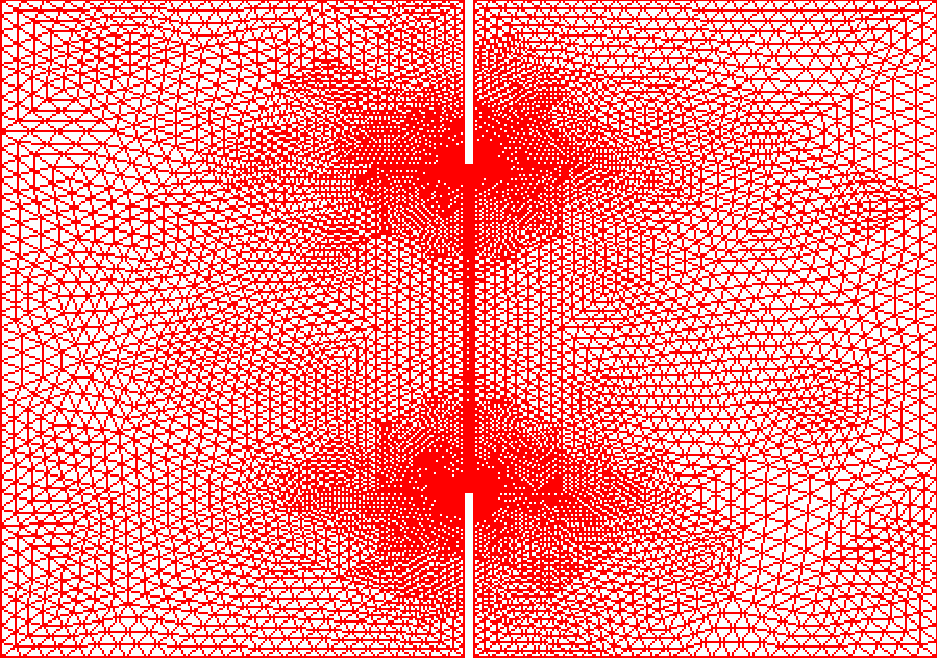
\includegraphics[width=8cm]{images/dambreak2dmesh.pdf}
\caption{Dominio di calcolo del problema del crollo della diga} \label{fig:dambreakdominio}
\end{figure}

Vediamo il programma. Si inizia includendo il modello (Shallow Waters), il flusso numerico di Lax-Friedrichs, il solutore a Volumi Finiti e il lettore della mesh.
\begin{lstlisting}[name=dambreak2d]
#include <models/shallowwater/shallowwater.hpp>
#include <solvers/fluxes/laxfriedrichs.hpp>
#include <solvers/finitevolume.hpp>
#include <mesh/io/meshreader.hpp>

#include <iostream>
#include <ctime>
#include <cmath>

using namespace std;
using namespace ConservationLaw2D;
\end{lstlisting}

A questo punto dobbiamo definire il solutore e tutto ciò che esso necessita. Da esso poi deriviamo la mesh, già particolareggiata per risolvere problemi con Volumi Finiti. Viene definito anche il tipo di soluzione, che sarà un vettore della giusta dimensione (grande tanto quante sono le variabili conservate, ossia 3). 
\begin{lstlisting}[name=dambreak2d]
typedef double real_t;
typedef Model::ShallowWater<real_t>              myModel;
typedef NumericalFlux::LaxFriedrichs<myModel>    myNumFlux;
typedef Solver::FiniteVolume<myModel,myNumFlux>  mySolver;
typedef mySolver::FVMesh                         myMesh;

// Tipo per la soluzione (vettore d-dim)
typedef myModel::SolType         SolType;
\end{lstlisting}
Definiamo ora le condizioni iniziali (nelle variabili primitive): a destra acqua alta, a sinistra acqua bassa.
\begin{lstlisting}[name=dambreak2d]
inline SolType init( size_t color, real_t x, real_t y ) {
    SolType sol = SolType::Zero();
    // rho, u, v
    sol[0] = ( x < 0 ) ? 4.0 : 1.0;
    sol[1] = 0.0;
    sol[2] = 0.0;
    return sol;
}
\end{lstlisting}
Analogamente per le condizioni al bordo (assorbenti nei lati esterni, di parete su quelle interne):
\begin{lstlisting}[name=dambreak2d]
inline SolType bc( SolType& wl, size_t color, real_t x, real_t y, real_t nx, real_t ny, real_t t ) {
    SolType wr = SolType::Zero();
    switch (color) {
        case 8:
        case 11:
        case 15:
        case 10:
        case 18:
        case 13:
            // Riflettente
            wr[0] = wl[0];
            wr[1] = (ny*ny-nx*nx)*wl[1] - 2*nx*ny*wl[2];
            wr[2] = - 2*nx*ny*wl[1] + (nx*nx-ny*ny)*wl[2];
            break;
        default:
           // Assorbente
           wr = wl;
           break;
    }
    return wr;
}
\end{lstlisting}
Come si osserva nella signature della funzione vengono passati lo stato a sinistra nelle variabili primitive wl, il colore del lato, le coordinate del punto medio, la normale e l'istante di tempo corrente.

Ora che ci sono tutti gli ingredienti si può inizializzare il problema:
\begin{lstlisting}[name=dambreak2d]
int main(int argc, char **argv) {
    // Parametri in ingresso
    bool gnuplot(false), interpolated(false);
    string meshfile;
    if ( argc < 2 ) {
        cout << "Usage: " << argv[0] << " [options] meshfile.msh" << endl;
        cout << "Options:" << endl;
        cout << "  --gnuplot\t\tGenerate plot and animation from gnuplot" << endl;
        cout << "  --interpolated\t\tInterpolate solution on vertices" << endl;
        exit(1);
    }
    for (int i=1; i<argc; ++i) {
        if (!strcmp(argv[i],"--gnuplot")) 
            gnuplot = true;
        else if (!strcmp(argv[i],"--interpolated"))
            interpolated = true;
        else
            meshfile = argv[i];
    }
    // Definisco il modello
    myModel model;
    // Definisco la mesh
    myMesh mesh;
    // Leggo la mesh
    Mesh::IO::MeshReader(mesh, meshfile);
    // Definisco il solutore per il mio modello
    mySolver solver(model, mesh);
    // Inizializzo alcuni parametri
    solver.setCFLmax(0.1);
    solver.setIC(init);
    solver.setBC(bc);
    solver.init();

    for (int i = 0; i < 1000; ++i) {
        std::cout << "== Timestep " << i << " == currtime: " << std::setw(8) << solver.getCurrTime();
        std::cout << ", dt = " << std::setw(8) << solver.getCurrDt() << std::endl;
        solver.timestep();
        if (i%50 == 0) solver.framegrab(i/50, gnuplot, interpolated);
    }
    return 0;
}
\end{lstlisting}
Nell'inizializzazione vengono automaticamente calcolate e salvate tutte le quantità geometriche fondamentali, per ottimizzare il solutore (linea 80). Nell'ultima parte invece viene fatto l'avanzamento in tempo vero e proprio.

L'esecuzione del programma è automatizzata attraverso lo script Perl postprocessing.py che richiede come argomento il file della mesh. 
Un output tipo è: 
\begin{verbatim}
>> Rimozione dati precedenti:   Fatto!
>> Simulazione:
=============================                      
Init Finite Volume Solver ...                      
=============================                      
== Timestep 0 == currtime:        0, dt = -0.0408514
== Timestep 1 == currtime: 8.61185e-05, dt = 8.61185e-05
== Timestep 2 == currtime: 0.000172237, dt = 8.61185e-05
[cut]
>> Genero frame 0:      Fatto!
>> Genero frame 1:      Fatto!
>> Genero frame 2:      Fatto!
[cut]
>> Genero animazione:   Fatto!
\end{verbatim}

Verrà rappresentata la soluzione in quattro istanti temporali successivi, in particolare si mostreranno l'andamento dell'altezza del fluido e il modulo della velocità (Figura \ref{fig:dambreak}).

\begin{figure}[htbp]
\centering
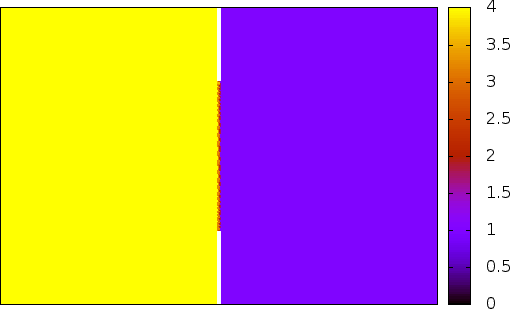
\includegraphics[width=0.4\textwidth]{images/DamBreak/height-solution0000.png} \hspace{0.2cm} 
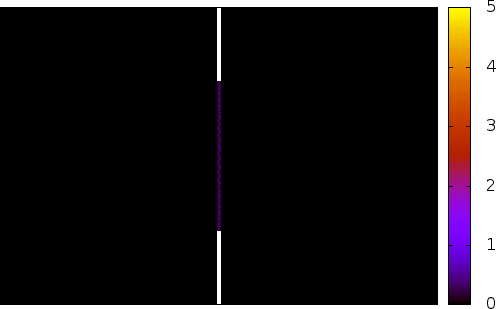
\includegraphics[width=0.4\textwidth]{images/DamBreak/velocity-solution0000.png} \\[0.5cm]
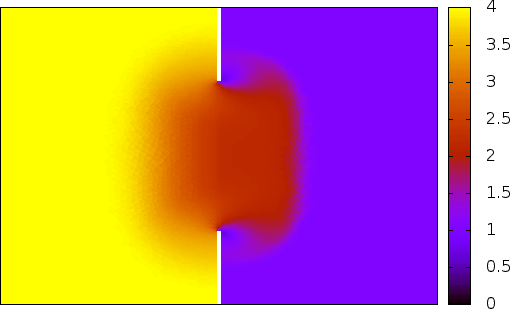
\includegraphics[width=0.4\textwidth]{images/DamBreak/height-solution0200.png} \hspace{0.2cm}
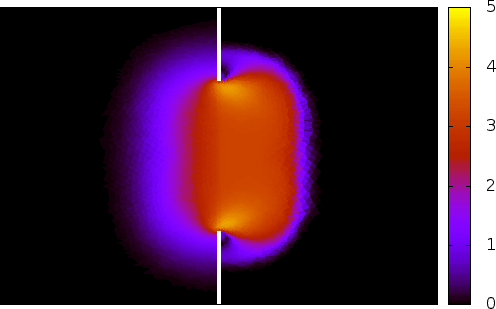
\includegraphics[width=0.4\textwidth]{images/DamBreak/velocity-solution0200.png}  \\[0.5cm] 
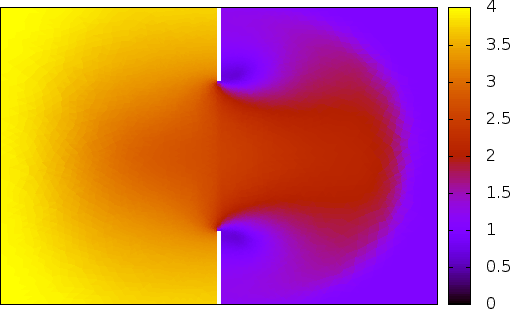
\includegraphics[width=0.4\textwidth]{images/DamBreak/height-solution0500.png}  \hspace{0.2cm}
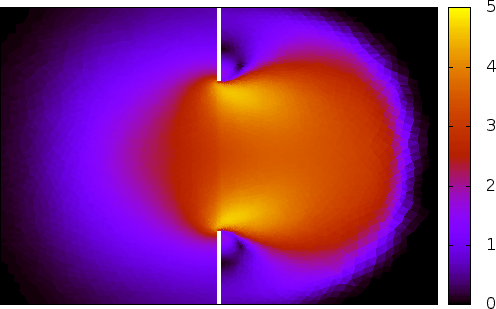
\includegraphics[width=0.4\textwidth]{images/DamBreak/velocity-solution0500.png}  \\[0.5cm]
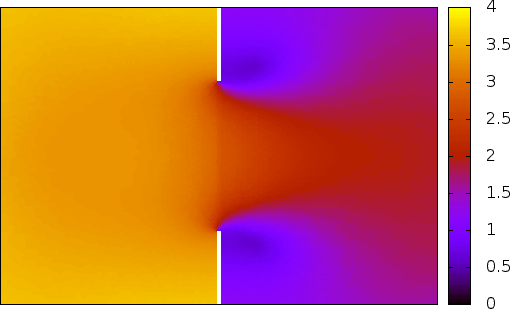
\includegraphics[width=0.4\textwidth]{images/DamBreak/height-solution0900.png}  \hspace{0.2cm}
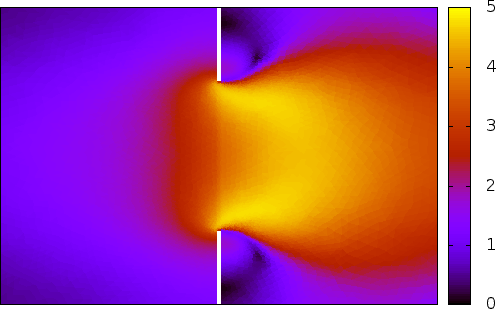
\includegraphics[width=0.4\textwidth]{images/DamBreak/velocity-solution0900.png}
\caption{Andamento dell'altezza (sinistra) e del modulo della velocità (destra) per il problema del crollo della diga con Lax-Friedrichs.}
\label{fig:dambreak}
\end{figure}

Questo test è molto semplice e lo schema ai Volumi Finiti riesce a cogliere con buona approssimazione tutti i fenomeni tipici del sistema. In particolare, notiamo che a valle della parete si generano zone di ricircolo e depressione che risultano ben definite. Inoltre, analizzando l'andamento del modulo di velocità, appare evidente l'aumento di velocità ai bordi dello sbocco e il successivo allargamento di vena a valle della diga.

Ovviamente la risoluzione è molto limitata dal fatto che stiamo utilizzando un metodo di ordine zero e un flusso numerico particolarmente dissipativo.

\subsection{Shock Bubble}
Presentiamo ora la soluzione ottenuta per il problema dello shock bubble, ovvero uno shock che investe una bolla di gas a densità minore. Lo schema numerico utilizzato è Roe con entropy fix. Viene mostrata la soluzione (rappresentata da densità e modulo della velocità) in quattro istanti temporali successivi (Figura \ref{fig:shockbubble}).
 
In particolare, il modello che regola il comportamneto del sistema è costituito dalle equazioni Eulero, che si ottiengono da quelle di Navier-Stokes considerando un fluido inviscido: si eliminano così tutti i contributi relativi alla viscosità e il sistema di equazioni si semplifica nel seguente modo:
\begin{equation} \label{eq:eulero}
\begin{cases}
&\pdd{\rho}{t} + \diverg \left(\rho \textbf{u}\right) = 0\\[1.5ex]
&\pdd{\left(\rho \textbf{u}\right)}{t} + \diverg \left(\rho \textbf{u} \otimes \textbf{u} + p \right) = \rho f^{V}\\[1.5ex]
&\pdd{\left(\rho e\right)}{t} + \diverg \left(\rho h \textbf{u} + \frac{1}{2} \rho |\textbf{u}|^{2} \textbf{u} \right) = \rho r + \rho f^{V} \textbf{u}
\end{cases}
\end{equation}
dove $\rho$ è la densità del fluido (non costante), $f^{V}$ sono le forze di volume agenti sul fluido, $e$ è l'energia specifica per unità di massa, $h$ è l'entalpia specifica e $r$ rappresenta un termine sorgente di calore per unità di massa e di tempo.  

Definendo il vettore delle incognite $\textbf{q} = \left[ \begin{matrix} \rho & \rho u & \rho v & \rho e \end{matrix} \right]^{\text{T}}$ il sistema \eqref{eq:eulero} si può scrivere in forma compatta in questo modo:
\begin{equation*}
\pdd{\textbf{q}}{t} + \pdd{\textbf{F}_{1}(\textbf{q})}{x} + \pdd{\textbf{F}_{2}(\textbf{q})}{y} = \textbf{S}(\textbf{q})
\end{equation*}
in cui $\textbf{S}(\textbf{q})$ rappresenta il vettore delle forzanti.
 
Tale relazione si può anche scrivere in forma quasi-lineare, il che permette di osservare nel nostro caso che si tratta di un problema \emph{iperbolico}: se si proietta questa equazione lungo una direzione $\nn$ si ottiene una matrice $\textbf{A}(\textbf{q};\nn)$ diagonalizzabile con tutti gli autovalori reali.
 
Nel caso di Eulero, gli autovalori della matrice $\textbf{A}(\textbf{q};\nn)$ sono infatti:
\begin{equation*}
\left\{ \begin{aligned}
\lambda_{1,4} &= \textbf{u} \cdot \nn \pm c \\[1.5ex]
\lambda_{2,3} &= \textbf{u} \cdot \nn
\end{aligned}  \right.
\end{equation*}
dove $c$ è la velocità locale del suono definita da $c = \sqrt{\partial{p}/\partial{\rho}}$. Possiamo osservare che l'autovalore $\lambda_{2,3}$ è degenere con molteplicità algebrica 2; le onde associate agli autovalori $\lambda_{1}$ e $\lambda_{4}$ sono onde sonore. Pertanto, alcune informazioni si propagano a velocità $\mathbf{u}\cdot\nn \pm c$ mentre altre sono trasportate dal flusso.

Per imporre le condizioni iniziali, il dominio di calcolo può essere diviso in tre zone: la prima zona è rappresentata dalla bolla, in cui $\rho = 0.1$, $p = 1$ , $u = v = 0 $; la seconda zona è quella a valle dello shock (bolla esclusa), in cui $\rho = 1$, $p = 1$ , $u = v = 0 $; mentre nella zona a monte della discontinuità si pone $p = 10$ mentre le altre grandezze si ricavano, essendo noti gli stati nelle altre zone. Le condizioni al bordo imposte sono tutte assorbenti.

\begin{figure}[htbp]
\centering
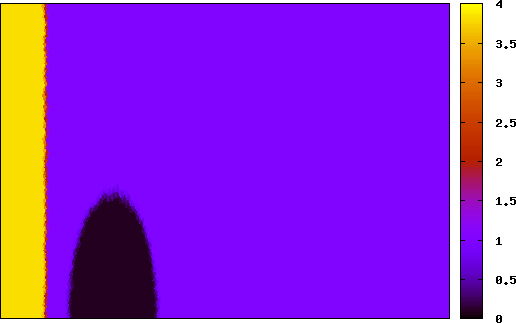
\includegraphics[width=0.4\textwidth]{images/ShockBubbleNew/height-solution0000bis.png} \hspace{0.2cm} 
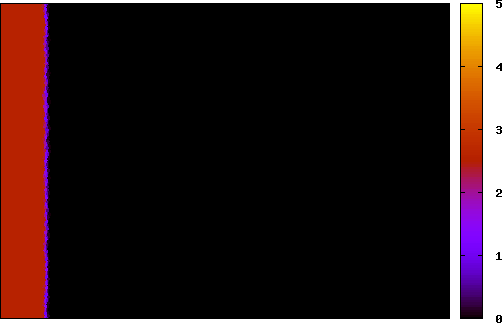
\includegraphics[width=0.4\textwidth]{images/ShockBubbleNew/velocity-solution0000bis.png} \\[0.5cm]
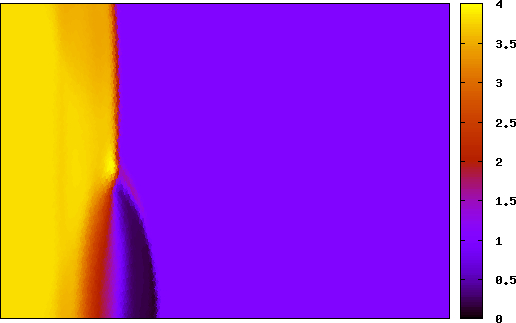
\includegraphics[width=0.4\textwidth]{images/ShockBubbleNew/height-solution0010bis.png} \hspace{0.2cm}
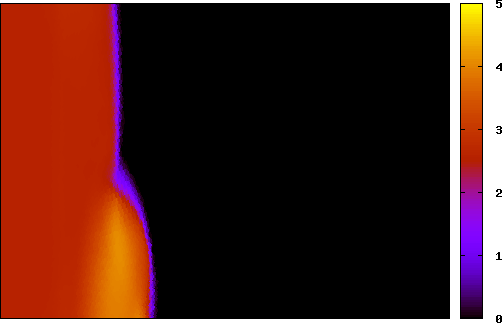
\includegraphics[width=0.4\textwidth]{images/ShockBubbleNew/velocity-solution0010bis.png}  \\[0.5cm] 
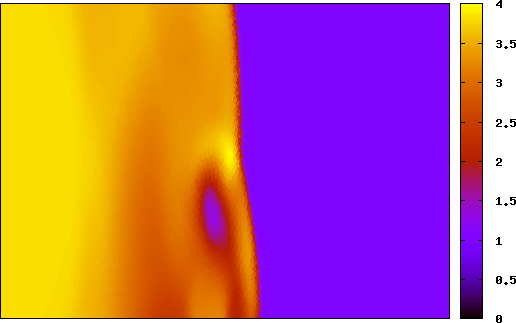
\includegraphics[width=0.4\textwidth]{images/ShockBubbleNew/height-solution0030bis.png}  \hspace{0.2cm}
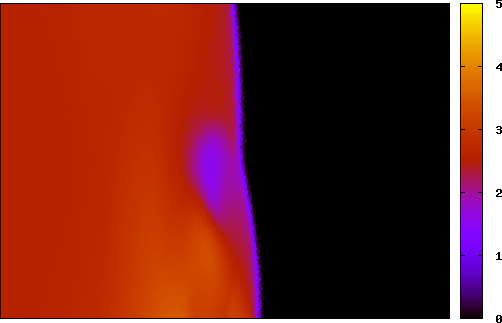
\includegraphics[width=0.4\textwidth]{images/ShockBubbleNew/velocity-solution0030bis.png}  \\[0.5cm]
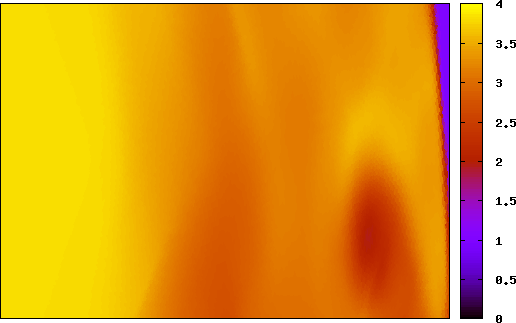
\includegraphics[width=0.4\textwidth]{images/ShockBubbleNew/height-solution0060bis.png}  \hspace{0.2cm}
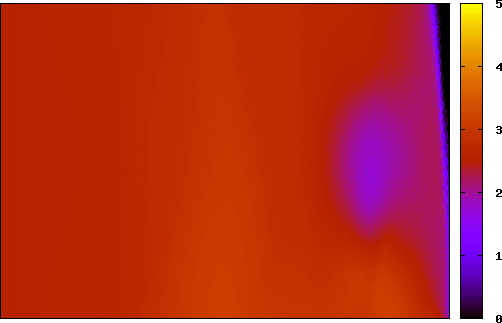
\includegraphics[width=0.4\textwidth]{images/ShockBubbleNew/velocity-solution0060bis.png}
\caption{Andamento della densità (sinistra) e del modulo della velocità (destra) per il problema shock bubble con Roe con entropy fix.}
\label{fig:shockbubble}
\end{figure}

La particolarità di questo esperimento (che alcuni ricercatori hanno anche eseguito realmente \cite{Williams1998307}) è che la bolla una volta investita dallo shock si avvolge su se stessa formando un toro: le immagini in Figura \ref{fig:shockbubble} devono essere pensate come una sezione di un volume a simmetria di rotazione.

Questo test numerico ci permette di osservare come il metodo dei Volumi Finiti necessiti di griglie molto fitte per ottenere risultati di buona qualità: in particolare, in questa simulazione si sono utilizzati circa 20000 triangoli, ma non sono stati sufficienti, infatti si sono persi molti dettagli interessanti dell'evoluzione del sistema (ad esempio, non sono definite molte zone di ricircolo e neanche le varie riflessioni che lo shock subisce).

\section{Conclusioni}
Lo schema a Volumi Finiti \eqref{eq:schemavolumifiniti} presenta caratteristiche molto particolari rispetto, per esempio, ad uno schema ad Elementi Finiti per la risoluzione di problemi ellittici.

La struttura è molto semplice ed intuitiva, nonché di semplice implementazione una volta che si ha a disposizione un buon gestore della mesh. Inoltre l'estensione al caso multidimensionale è praticamente automatica, se non per alcuni dettagli riguardanti la geometria. Al contrario un codice FEM presenta certamente difficoltà aggiuntive dovute alla presenza di integrazione numerica, costruzione di matrici sparse, risoluzione di sistemi lineari, e via discorrendo.

Il problema principale però è che sistemi iperbolici tipo Eulero sono estremamente più complessi rispetto a problemi ellittici e parabolici, e tutta questa complessità si riflette poi nelle soluzioni approssimate generate dal metodo numerico. Infatti nei sistemi iperbolici la regolarità delle soluzioni è una questione spinosa, proprio perché manca il termine diffusivo che tende a smussare le discontinuità. Il metodo dei Volumi Finiti, di ordine basso per via dell'approssimazione costante a tratti della soluzione, è adatto quindi dove la regolarità della soluzione non consente un ordine elevato di convergenza, mentre mostra i suoi limiti dove invece la soluzione è più regolare.

Nel problema Shock Bubble molti dettagli non sono stati colti adeguatamente. Eventuali modifiche per migliorare questo aspetto possono però andare in queste direzioni:
\begin{itemize}
\item \emph{Adattività di griglia}, che permetterebbe di concentrare i nostri sforzi computazionali solo vicino alle discontinuità (o a zone con forti gradienti);
\item \emph{Limitatori di pendenza}, con i quali, attraverso particolari procedure (abbastanza complesse nel caso di griglie non strutturate), si ricostruisce una approssimazione lineare della soluzione in ogni elemento, e si utilizzano poi le tracce al bordo di quest'ultima per calcolare i flussi numerici. La particolarità è che per evitare eventuali oscillazioni spurie dovute alla ricostruzione di ordine più elevato si possono costruire limitatori di pendenza (del tutto analoghi al caso 1D) che attivano la ricostruzione solo se necessario. L'ordine di convergenza del metodo così ottenuto risulterà essere più elevato rispetto a quello originale, almeno lontano dalle discontinuità (ove non si può comunque far di meglio);
\item \emph{Metodo Discontinous Galerkin}, il quale cerca di conciliare i punti di forza del metodo dei Volumi Finiti con quello degli Elementi Finiti. In questo caso la soluzione in ogni elemento è combinazione lineare di funzioni di base, e dunque ad ogni passo temporale e su ogni triangolo si deve risolvere un sistema lineare. Lo scopo di tutto ciò è quello di ottenere una approssimazione migliore utilizzando meno triangoli, almeno nelle zone in cui la soluzione è regolare. Ovviamente la generalizzazione è immediata solo a parole, in quanto diventano necessarie a questo punto procedure per l'assemblaggio delle matrici, per l'integrazione numerica, per l'interpolazione e via dicendo.
\end{itemize}

Da un punto di vista del codice, l'implementazione di queste estensioni non comporta drastiche modifiche allo stesso. Ad esempio per il metodo Discontinous Galerkin si possono estendere le classi \texttt{BasePolygon} e \texttt{BaseHEdge} in modo tale che siano disponibili dei metodi per l'integrazione sul poligono o sul lato. Per la risoluzione del sistema lineare si può ricorrere a classi esterne di algebra lineare\footnote{Il codice fa uso della libreria \texttt{Eigen} (\url{http://eigen.tuxfamily.org}), la quale mette a disposizione una vasta gamma di classi e metodi per l'algebra lineare.}, richiamate poi direttamente dal solutore. Anche i limitatori di pendenza richiedono poche modifiche strutturali.

Per quanto riguarda l'adattività di griglia invece possono esserci più problemi, perché in questo caso (a meno di rigenerare ogni volta la mesh da zero) si deve metter mano alla struttura dati. Eliminare un triangolo per poi aggiungerne di più piccoli non è certamente una procedura efficiente, piuttosto si dovrebbe lavorare direttamente sui puntatori della struttura dati.

Nello sviluppo del codice si è optato per un largo utilizzo di \emph{templates}, in modo da ottimizzare il più possibile il codice ed allo stesso tempo mantenere un buon livello di astrazione. Questa scelta ha reso lo sviluppo molto problematico e lento, soprattutto per quanto concerne la gestione della mesh, ma ha poi permesso uno sviluppo del solutore molto più rapido ed intuitivo.

Tra le scelte un pò meno lungimiranti nello sviluppo possiamo certamente evidenziare il caso della gestione delle condizioni iniziali e al bordo, che poteva essere affrontata in modo più elegante attraverso l'utilizzo di funtori. Oppure anche la scelta di conservare la soluzione direttamente nella struttura dati del poligono piuttosto che elevare il livello di astrazione definendo delle classi per lo spazio funzionale. Queste scelte sono di pura convenienza, e non trovano una valida giustificazione, se non il fatto che ``così è più semplice''. Inoltre, ogni codice buon Open Source che si rispetti non pone mai la frase ``versione definitiva'' tra le righe del suo sorgente.
\newpage
% BIBLIO
\begin{bibdiv}
\begin{biblist}
\bibselect{biblio}
\end{biblist}
\end{bibdiv}
% APPENDICE
\newpage
\appendix
\section{Flussi numerici} \label{app:flussinum}
Nello schema \eqref{eq:schemavolumifiniti} resta ancora da scegliere il flusso numerico $\NumFlux(\mathbf U^n_i, \mathbf U^n_j, \nn_{ij})$, il quale deve soddisfare le seguenti proprietà:
\begin{enumerate}
\item $\abs{\NumFlux(u, v, \nn_{ij}) - \NumFlux(u', v', \nn_{ij}) } \le C \max_i \diam K_i \bigl( \abs{u-u'} + \abs{v-v'} \bigr)$;
\item $\NumFlux(u, v, \nn_{ij}) = - \NumFlux(v, u, \nn_{ji})$;
\item $\NumFlux(u, u, \nn_{ij}) = \Flux(u; \nn_{ij})$.
\end{enumerate}
La prima è una condizione di Lipschitzianità, la seconda indica che il flusso è conservativo, mentre l'ultima è una relazione di consistenza.

Come già osservato, in direzione normale il problema è essenzialmente monodimensionale: possiamo quindi utilizzare flussi numerici già noti.
\subsection{Metodo di Lax-Friedrichs}
Il metodo di Lax-Friedrichs utilizza un flusso del tipo:
\begin{equation*}
\NumFlux(\mathbf U_i, \mathbf U_j, \nn_{ij}) = \frac{1}{2} \left[ \Flux(\mathbf U_i; \nn_{ij}) + \Flux (\mathbf U_j; \nn_{ij}) \right] - \frac{c}{2} \left( \mathbf U_j - \mathbf U_i \right)
\end{equation*}
dove $c = \max \bigl\{ \abs{\lambda(\mathbf U_i)}, \abs{\lambda(\mathbf U_j)} \bigr\}$ è la massima velocità di propagazione delle onde.

L'implementazione di questo flusso numerico è molto semplice, a costo però di un'eccessiva dissipazione numerica che vicino alle discontinuità tende a smussare gli angoli.
\subsection{Metodo di Godunov}
L'idea alla base del metodo è quella di risolvere esattamente su ogni lato un problema di Riemann con onde piane nella direzione $\nn_{ij}$, con dati $\mathbf{U}_i$ e $\mathbf{U}_j$. Sarà quindi:
\begin{equation*}
\NumFlux(\mathbf{U}_i, \mathbf{U}_j, \nn_{ij} ) = \Flux( \tilde{\mathbf{U}}_{ij}(0); \nn_{ij} )
\end{equation*}
dove $\tilde{\mathbf{U}}_{ij}\left( \frac{\left(\mathbf{x}-\mathbf{m}_{ij}\right) \cdot \nn_{ij}}{t}\right)$ è la soluzione esatta del problema di Riemann all'interfaccia e $\mathbf{m}_{ij}$ è invece il punto medio del lato su cui si sta lavorando.
\subsection{Flussi numerici approssimati}
Spesso applicare in modo rigoroso il metodo di Godunov risulta troppo oneroso. Per questo si opta per flussi numerici approssimati, i quali spesso mostrano performances simili a quelle dei solutori esatti.

In letteratura è presente una grande varietà di flussi approssimati, i quali si basano sull'idea di sostituire al flusso esatto una funzione che approssimi la vera soluzione del problema di Riemann con gli stessi dati iniziali. Uno dei solutori più noti è quello di Roe.

Altre tipologie di flussi approssimati, come Rusanov, HLL e HLLC, modificano direttamente il flusso numerico con correzioni adeguate. Questi metodi (così come Roe) necessitano però di una taratura, ossia alcuni parametri che descrivono lo stato del sistema devono essere opportunamente stimati, ad esempio attraverso delle medie particolari.

In particolare, nel caso del problema di Eulero, possiamo utilizzare le seguenti forme esplicite dei flussi citati:
\begin{align*}
\NumFlux &= \frac{1}{2}(\NumFlux_L + \NumFlux_R) - \frac{1}{2} S^+ (\textbf{U}_R - \textbf{U}_L) & \text{(Rusanov)} \\[2ex]
\NumFlux^{\text{hll}} &= 
\begin{cases}
\NumFlux_L & \text{se $0 \leq S_L$} \\[2ex]
\dfrac{S_R\NumFlux_L - S_L\NumFlux_R + S_L S_R (\textbf{U}_R -\textbf{U}_L)}{S_R - S_L} & \text{se $S_L \leq 0 \leq  S_R$} \\[2.5ex]
\NumFlux_R & \text{se $0 \geq S_R$}
\end{cases} & \text{(HLL)} \\[2ex]
\NumFlux^{\text{hllc}} &= 
\begin{cases}
\NumFlux_L & \text{se $0 \leq S_L$} \\
\NumFlux_L + S_L (\textbf{U}_{*L} - \textbf{U}_L ) & \text{se $S_L \leq 0 \leq S_*$}\\
\NumFlux_R + S_R (\textbf{U}_{*R} - \textbf{U}_R ) & \text{se $S_* \leq 0 \leq S_R$}\\
\NumFlux_R & \text{se $0 \geq S_R$}
\end{cases} & \text{(HLLC)}
\end{align*}
dove $S^+ = \text{max} \left\{\left|u_L\right| + c_L, \left|u_R\right| + c_R \right\}$, $S_L$ e $S_R$ sono le velocità di propagazione dell'informazione relative alle due onde esterne, $\textbf{U}_L$ e $\textbf{U}_R$ sono gli stati di sinistra e di destra, $S^*$ è la velocità dell'onda centrale (quella nella cosiddetta zona star), quella corrispondente all'autovalore multiplo, mentre $\textbf{U}_{*L}$ e $\textbf{U}_{*R}$ sono opportune stime dello stato del sistema nella zona star.

Infine, il metodo di Roe si basa sull'utilizzo di opportune medie delle variabili che descrivono lo stato del sistema:
\begin{equation*}
\begin{aligned}
\tilde{u} &= \frac{\sqrt{\rho_L} u_L + \sqrt{\rho_R} u_R}{\sqrt{\rho_L} + \sqrt{\rho_R}}; 
&&\tilde{v} = \frac{\sqrt{\rho_L} v_L + \sqrt{\rho_R} v_R}{\sqrt{\rho_L} + \sqrt{\rho_R}}; \\
\tilde{H} &= \frac{\sqrt{\rho_L} H_L + \sqrt{\rho_R} H_R}{\sqrt{\rho_L} + \sqrt{\rho_R}}; 
&&\tilde{c} = (\gamma - 1) \left[\tilde{H} - \frac{1}{2} \tilde{V}^{2} \right] ^{1/2}.
\end{aligned}
\end{equation*}
Con i pedici L e R si sono indicati i valori della relativa grandezza a destra e a sinistra; $\tilde{H}$ è l'entalpia e $\tilde{V}$ è il modulo della velocità mediata.
Tali grandezze servono per definire un sistema linearizzato la cui soluzione descrive l'evoluzione del sistema. E' poi possibile correggere lo schema di Roe aggiungendo un fix entropico in modo tale da garantire che lo schema legga correttamente le onde di rarefazione transoniche.
\section{Formato dei file}
Vi sono essenzialmente tre formati di file che il programma utilizza: uno riguardante la descrizione della mesh e due per l'output delle soluzioni.

Riguardo la mesh, il file ha una forma di questo tipo:
\begin{verbatim}
# DATA
133     218     54
# POINTS
-1.000000       0.500000
-1.000000       -0.500000
0.000000        -0.200000
[cut]
-0.063683       0.163276
0.163695        -0.167380
-0.069532       -0.241330
# ELEMENTS
3       15      1       58      1
3       22      2       61      0
[cut]
3       104     112     132     1
3       2       126     132     1
# EDGES
0       12      0
12      13      0
13      14      0
[cut]
50      51      13
51      11      13
\end{verbatim}
Il file è suddiviso in quattro sezioni:
\begin{description}
\item[\texttt{\# DATA}] Le tre colonne indicano rispettivamente il numero di vertici, di poligoni e di lati di bordo;
\item[\texttt{\# POINTS}] Ogni riga è un vertice, del quale vengono fornite le coordinate;
\item[\texttt{\# ELEMENTS}] Ogni riga è un poligono, e le colonne sono rispettivamente il numero di lati, l'id dei vertici (in senso antiorario) ed infine il colore dell'elemento;
\item[\texttt{\# EDGES}] Ogni riga è un lato di bordo, del quale si forniscono i vertici e il colore.
\end{description}

Un file di questo tipo può essere facilmente generato in Matlab utilizzando \texttt{matlab2msh.m}, script presente nella directory \texttt{tools}. Da un punto di vista pratico ci si appoggia al toolbox \texttt{pdetool}, col quale genera mesh (il risultato dovrebbero essere tre variabili \texttt{p}, \texttt{e} e \texttt{t}), per poi eseguire:
\begin{verbatim}
>> matlab2msh(p,e,t,'nomefile.msh');
\end{verbatim}
Automaticamente come etichette \texttt{colore} dei poligoni e dei lati vengono assegnate ``d'ufficio'' rispettivamente l'id del sottodominio e l'id del bordo. Attraverso l'interfaccia grafica di \texttt{pdetool} è anche possibile visualizzare queste etichette.

Per quanto riguarda l'output su file della soluzione, come accennato ci sono due formati, il primo per l'output grafico in Matlab mentre il secondo per l'output in Gnuplot.

Nel primo caso si ha semplicemente una lista di valori, dove ogni riga è il valore della soluzione nel vertice corrispondente, secondo lo stesso ordinamento del file della mesh in input. Vi sono inoltre tante colonne quante sono le variabili del problema (4 per Eulero).

La soluzione è automaticamente interpolata sui vertici, e si può visualizzare in Matlab importando il file in una variabile e utilizzando poi i comandi \texttt{pdeplot} o \texttt{trisurf}. Sempre nella directory \texttt{tools} vi sono alcuni esempi pratici, come la generazione di una animazione.

L'ultimo formato riguarda il dataset della soluzione pronto per essere utilizzato in Gnuplot attraverso il comando \texttt{splot}\footnote{Nella visualizzazione tridimensionale potrebbe esserci della grafica corrotta, probabilmente perché il comando è disegnato per utilizzare dataset con griglie cartesiane. Nel nostro caso infatti per rappresentare i triangoli costruiamo dei quadrilateri degeneri.}. In questo caso si può decidere se interpolare la soluzione sui vertici oppure no.
\end{document}